%%
%% Author: Gerard Bosch (gerard.bosch@gmail.com)
%% 13/02/2018
%%

\documentclass[notitlepage, usenames,dvipsnames]{beamer}
\usefonttheme[onlymath]{serif}      %font serif (beamer usa sans-serif) per a l'entorn math
\usepackage{beamerprosper}
\usepackage{pstricks-add}
%\usepackage{beamertexpower}
\usepackage[utf8]{inputenc}
\usepackage[english]{babel}
%\usepackage{default}
\usepackage{verbatim}
\usepackage{multicol}
\usepackage{graphicx}

%\setbeameroption{show notes on second screen=right}
\setbeamertemplate{navigation symbols}{}

%% Aliases %%
\renewcommand{\tt}{\texttt}     %redefinit! és l'entorn typewriter, però sempre faig anar verbatims.
\newcommand{\ts}{\textsl}
\renewcommand{\ni}{\noindent}   %redefinit! és un simbol de math, \in al revés :S
\newcommand{\eh}{\emph}
\newcommand{\st}{\structure}


\usetheme[secheader]{Boadilla}
%\usetheme{Copenhagen}
%\usetheme{Darmstadt}
%\usetheme{Frankfurt}
%\usetheme{Goettingen}
%\usetheme{Hannover}
%\usetheme{Luebeck}
%\usetheme[secheader]{Madrid}
%\usetheme{Warsaw}


%\setbeamercolor{frametitle}{bg=gray!10}
%\setbeamercolor{block body alerted}{bg=red!20}
%\setbeamercolor{frametitle}{use=structure,bg=structure.fg!10!bg}
%\setbeamercolor{frametitle}{parent=normal text,use=block title,bg=block title.bg!50!bg}


%\hypersetup{pdfpagemode=FullScreen}


\title[Introduction to Blockchain Technology]{An introduction to Blockchain technology}
%\subtitle{}
\author[Gerard Bosch]{Gerard Bosch}
\institute{\email{gerard.bosch@gmail.com}}
\date{\today}

% \AtBeginSection[]{\frame[shrink]{\frametitle{Outline}\tableofcontents[currentsection]}} %posar [*] per aplicar-ho a \section*
\AtBeginSection[]{\frame{\frametitle{Outline}\begin{multicols}{2} \tableofcontents[currentsection] \end{multicols}}}    % 2 columns toc

% 2 columns table of contents !package multicol
% \begin{frame}
% \begin{multicols}{2}
%   \tableofcontents
% \end{multicols}
% \end{frame}

\setbeamercovered{transparent}


\begin{document}


%%%%%%%%%%%%%%%%%%%%% Custom title %%%%%%%%%%%%%%%%%%%%%
\begin{frame}
\begin{center}
\vspace{-4mm}\begin{center}
\includegraphics[scale=0.15]{../img/gft.jpg}\end{center}

%\rule{\linewidth}{1.5pt} \\[3mm]
\vspace{1cm}
{\huge \bfseries \textcolor{MidnightBlue!100!bg}{ An introduction to\\[3mm] Blockchain technology }} \\[3mm]
%\rule{\linewidth}{1.5pt} \\[3mm]

\vspace{1 cm}
Gerard Bosch (gerard.bosch@gmail.com)

\vspace{0.8cm}\today
\end{center}
\end{frame}
%%%%%%%%%%%%%%%%%%%%%% End title %%%%%%%%%%%%%%%%%%%%%%%



%\maketitle
\frame[shrink]{\frametitle{Outline}\tableofcontents[hideallsubsections]}


\section{Preliminary concepts}
%--------------------------------Frame---------------------------------
\begin{frame}
    \frametitle{What is a Blockchain?}

    \begin{overlayarea}{\textwidth}{\textheight}

    \vspace{3ex}

    \begin{itemize}
    \itemsep=1.35ex
        \item A \alert{distributed cryptographic ledger} shared amongst all nodes participating in a network, over which every transaction is recorded.
        \item<5-> Blockchain serves as the \alert{underlying} technology of several \st{cryptocurrencies} such as Bitcoin.
        \item<7-> The concept and its implementation was created in 2009 and announced in a 9 pages paper writen by Satoshi Nakamoto.
    \end{itemize}

    \only<2> {
        \begin{exampleblock}{Ledger}
            The \st{foundation of accounting}, are as ancient as writing and money.
        \end{exampleblock}
    }

    \only<3> {
        \begin{exampleblock}{Cryptographic}
            The procedures and protocols to \st{append} new data to the ledger implies the use of cryptographic techniques.
        \end{exampleblock}
    }

    \only<4> {
        \begin{exampleblock}{Distributed}
            Not a single entity is the owner of the data, but it is \st{replicated} in every participant of the network.
        \end{exampleblock}
    }

    \only<6> {
        \begin{exampleblock}{Bitcoin}
            was the first and most popular \st{\eh{peer-to-peer} value exchange} network.
        \end{exampleblock}
    }

    \only<8> {
        \begin{exampleblock}{Satoshi Nakamoto}
            is a pseudonym of an anonymous individual or group that developed the idea of Blockchain and Bitcoin.
        \end{exampleblock}
    }

    \end{overlayarea}
\end{frame}
%--------------------------------End-----------------------------------


%--------------------------------Frame---------------------------------
\begin{frame}
    \frametitle{What is a Blockchain?}

    \begin{overlayarea}{\textwidth}{\textheight}

    \vspace{4ex}

    \only<1-> {
        \centering \Large Now we know, but\ldots how does it look like?
    }

    \only<2-> {
        \vspace{4ex}
        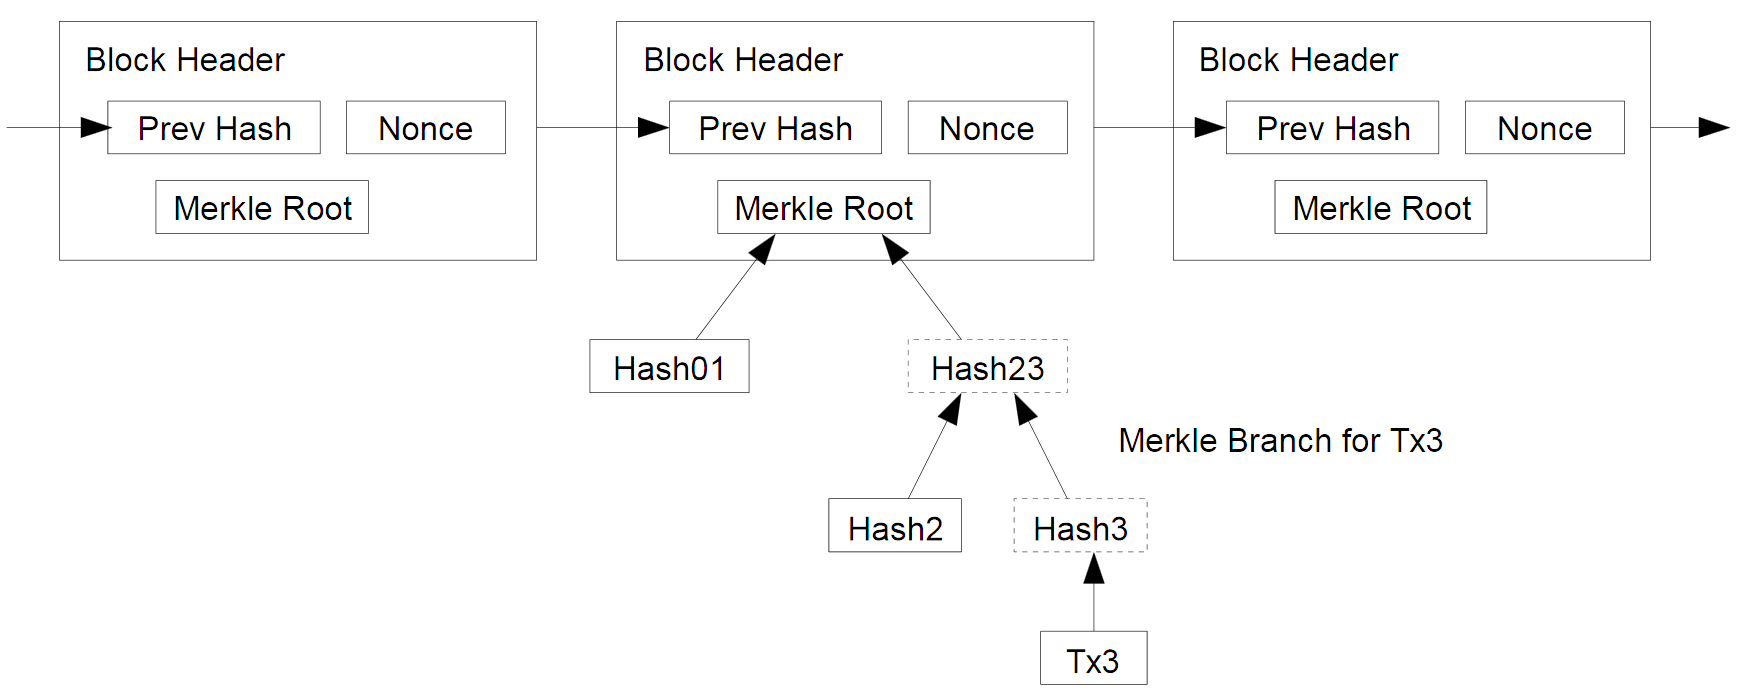
\includegraphics[scale=0.26]{../img/block-chain.png}
    }

    \end{overlayarea}
\end{frame}
%--------------------------------End-----------------------------------


%--------------------------------Frame---------------------------------
\begin{frame}
    \frametitle{A bit more background}

    \begin{itemize}
        \item Since Bitcoin appearance in 2009, several other \st{cryptocurrencies} emerged.
        \pause
        \item Currently most of them are based in some kind of Blockchain.
        \pause
        \item Blockchain provides a reliable infrastructure that provides \st{at least} 2 out of the 3 properties of \st{CIA triad}: \alert{integrity} and \alert{availability}.
    \end{itemize}

    \begin{exampleblock}{Integrity}<4->
        The use of asymetric cryptography guarantees the integrity of data.
    \end{exampleblock}

    \begin{exampleblock}{Availability}<5->
        As a decentralized network, there is no single point of failure.
    \end{exampleblock}

    \begin{block}{Confidentiality}<6->
        Some implementations seems that could provide it as well (ZCash?).
    \end{block}

\end{frame}
%--------------------------------End-----------------------------------

\section{How does it work?}
\subsection{Consensous}
%--------------------------------Frame---------------------------------
\begin{frame}
    \frametitle{How does it work?}

    \begin{overlayarea}{\textwidth}{0.7\textheight}

    \only<1-> {
        \begin{center}
            \LARGE \ts{``It is all about consensous''}
        \end{center}
    }

    \only<2-6> {
        \begin{itemize}\itemsep=1ex
            \pause
            \item Blockchain concept is in continuous \st{evolution} and new protocols are continuously created to improve the current flaws.
            \pause
            \item Earliest implementations (which includes Bitcoin and Ethereum) are using a system called \eh{Proof of Work} (\st{PoW}) to \alert{validate} the transactions.
            \pause
            \item \st{Validation} is required in order to append a new block of transactions to the chain; preventing things such as double spend.
            \pause
            \item The process of block validation is known as \st{mining}.
            \pause
            \item Lately a new system called \ts{Proof of Stake} (\st{PoS}) was developed to address PoW drawbacks.
        \end{itemize}
    }

    \only<7-> {
        \begin{itemize}\itemsep=1ex
            \item<7-> Nodes are motivated to maintain the network with a \st{reward} coming from transaction fees.
            \item<8-> Hence, \alert{consensus} is achieved though these systems.
        \end{itemize}
    }

    \end{overlayarea}
\end{frame}
%--------------------------------End-----------------------------------


%--------------------------------Frame---------------------------------
\begin{frame}
    \frametitle{Transaction workflow}

    \begin{enumerate}\itemsep=4ex
        \item Clients creates and \alert{signs} transactions (TX) using its private key, then they \st{broadcasts} TX to the network.
        \item Network nodes (miners) receives transactions and stores them in the so called \st{mempool}.
        \item Miners prioritize transactions based on fees and validate it.
        \item Once successfully validated a block is appended to the block chain.
    \end{enumerate}

\end{frame}
%--------------------------------End-----------------------------------


%--------------------------------Frame---------------------------------
\begin{frame}
    \frametitle{}

    \begin{center}
        \LARGE But how does it work under the hood?
    \end{center}

\end{frame}
%--------------------------------End-----------------------------------


\subsection{Proof of Work}
%--------------------------------Frame---------------------------------
\begin{frame}
    \frametitle{Proof of Work: The Bitcoin case}
    \begin{overlayarea}{\textwidth}{\textheight}

    \only<1-2> {
    \vspace{2ex}
    \begin{exampleblock}{Block mining}
        Participants of a Blockchain network put some \alert{resources} to validate transactions by \alert{solving} the so called \st{cryptographic puzzles}.
    \end{exampleblock}
    }

    \only<2> {
        \begin{itemize}\itemsep=1ex
            \item Block validation consist in finding a \st{nonce} (number) for the block that \st{satisfies} a property of the block's hash (a number of leading zeroes).
            \item This is a trial and error procedure (a kind of brute-force).
            \item The first node that find a successful solution \st{announce} it to the network.
            \item The rest of the nodes can \alert{easily verify} that the solution (and hence the block) is valid.
            \item If a node acts \alert{dishonestly}, the rest of nodes will discard the block.
        \end{itemize}
    }

%    \visible<3> {
%        \begin{block}{How?}
%            Taking the solution (nonce) into the block and computing block's hash (SHA-256) must result in a hash with a leading number of zeroes.\\
%            This is easy to verify for any node.
%        \end{block}
%    }

    % Drawbacks
    \only<3> {
        \vspace{2ex}
        \begin{alertblock}{Drawbacks}
            \begin{itemize}
                \item Huge energy consumption.
                \item Susceptible to a 51\% attack.
                \item Democratization of the network (hardware, electricity price,\ldots)
            \end{itemize}
        \end{alertblock}
    }

    \end{overlayarea}
\end{frame}
%--------------------------------End-----------------------------------


%--------------------------------Frame---------------------------------
\begin{frame}
    \frametitle{Proof of Stake}

    Given the aforementioned problems that PoW presents, the new model Proof of Stake was developed.

    \begin{itemize}
        \item In PoS, the resource the miner puts is an amount of currency it holds: the stake (a kind of deposit).
        \item The next block creator will be chosen randomly.
        \item % If the miner behaves dishonestly they lose the stake.
    \end{itemize}

    \begin{exampleblock}{Pros}
        \begin{itemize}
            \item Executing an attack would be much more expensive: Purchasing more than half of the coins is likely more costly than acquiring 51\% of PoS hashing power.
            \item
            \item
        \end{itemize}
    \end{exampleblock}

\end{frame}
%--------------------------------End-----------------------------------


%--------------------------------Frame---------------------------------
\begin{frame}
    \frametitle{}

\end{frame}
%--------------------------------End-----------------------------------


%--------------------------------Frame---------------------------------
\begin{frame}
    \frametitle{}

\end{frame}
%--------------------------------End-----------------------------------


%--------------------------------Frame---------------------------------
\begin{frame}
    \frametitle{}

\end{frame}
%--------------------------------End-----------------------------------


%--------------------------------Frame---------------------------------
\begin{frame}
    \frametitle{}

\end{frame}
%--------------------------------End-----------------------------------


%--------------------------------Frame---------------------------------
\begin{frame}
    \frametitle{}

\end{frame}
%--------------------------------End-----------------------------------


%--------------------------------Frame---------------------------------
\begin{frame}
    \frametitle{}

\end{frame}
%--------------------------------End-----------------------------------


%--------------------------------Frame---------------------------------
\begin{frame}
    \frametitle{}

\end{frame}
%--------------------------------End-----------------------------------


%--------------------------------Frame---------------------------------
\begin{frame}
    \frametitle{}

\end{frame}
%--------------------------------End-----------------------------------


%--------------------------------Frame---------------------------------
\begin{frame}
    \frametitle{}

\end{frame}
%--------------------------------End-----------------------------------


%--------------------------------Frame---------------------------------
\begin{frame}
    \frametitle{}

\end{frame}
%--------------------------------End-----------------------------------


%--------------------------------Frame---------------------------------
\begin{frame}
    \frametitle{}

\end{frame}
%--------------------------------End-----------------------------------


%--------------------------------Frame---------------------------------
\begin{frame}
    \frametitle{}

\end{frame}
%--------------------------------End-----------------------------------






\end{document}


%--------------------------------Frame---------------------------------
\begin{frame}
    \frametitle{}

\end{frame}
%--------------------------------End-----------------------------------